\documentclass[10pt]{beamer}	
%\documentclass[10pt,aspectratio=43,mathserif]{beamer}		
%设置为 Beamer 文档类型,设置字体为 10pt,长宽比为16:9,数学字体为 serif 风格
%\documentclass[handout]{beamer}

\usepackage{seu}
\usepackage{amsmath,amsfonts,amssymb,bm}
\usepackage{color}
\usepackage{graphicx,hyperref,url}
\usepackage[main=english]{babel} 

\title[\textbf{Map Reduce}]{\textbf{Map Reduce}}
\subtitle{\textbf{Experiment summary}}
\author{\textbf{Wu Qingyan}}

\institute[CSE@SEU]{{213221715@seu.edu.cn}}

\date{\scriptsize \today}

\usepackage{tikz}
\usetikzlibrary{calc, shapes, backgrounds}

% used within this chapter
\usepackage{marvosym}
\usepackage{listings}
\usepackage{xcolor}
\definecolor{mygreen}{rgb}{0,0.6,0}
\definecolor{mygray}{rgb}{0.5,0.5,0.5}
\definecolor{mymauve}{rgb}{0.58,0,0.82}
\lstset{basicstyle=\tiny, breaklines=true, numbers=left, numberstyle=\tiny\color{mygray}, keywordstyle=\color{blue}, commentstyle=\color{mygreen}, frame=shadowbox, rulesepcolor=\color{black}, stringstyle=\color{mymauve}, xleftmargin=2em, xrightmargin=2em, aboveskip=0em, language=C,showstringspaces=false}
\usepackage{pgfgantt}
\usepackage{adjustbox}
\usepackage[normalem]{ulem}
\usepackage{multirow}

\setbeamertemplate{itemize/enumerate body begin}{\footnotesize}
\setbeamertemplate{itemize/enumerate subbody begin}{\footnotesize}
\setbeamertemplate{itemize/enumerate subsubbody begin}{\footnotesize}

\begin{document}

\begin{frame}[label=title]
    \titlepage{}
\end{frame}

\AtBeginSection[]{
    \begin{frame}<beamer>
        \frametitle{Contents}
        \tableofcontents[
            sectionstyle=show/shaded,
            subsectionstyle=show/shaded
        ]
    \end{frame}}

\section[1.Intro]{What is MapReduce}
\begin{frame}{What is MapReduce}
    \framesubtitle{Introduction}
    \begin{itemize}
        \item MapReduce is a programming model for large-scale data processing.
              \note[item]{like word count, log analysis, etc.}
        \item Originally introduced by Google engineers.
        \item Enables parallel computation on distributed clusters.
              \note[item]{It enables parallel computation on large data sets in a distributed environment.}
        \item Developers focus on writing small code snippets.
              \note[item]{instead of writing complex parallel code by themselves.}
    \end{itemize}
\end{frame}

\section[2. Building a Simplified MapReduce]{Building a Simplified MapReduce}
\begin{frame}{Building a Simplified MapReduce}
    \framesubtitle{Introduction}
    \begin{itemize}
        \item In this project, we will construct a simplified version of MapReduce for a single machine.The challenge is how to implement correct concurrency support.This task has three specific objectives:

              \begin{enumerate}
                  \item Understand the general properties of the MapReduce paradigm.
                        \note[item]{paradgm: a typical example or pattern of something; a model.}
                  \item Implement a correct and efficient MapReduce framework using threads and relevant functions.
                  \item Gain more experience in writing concurrent code.
              \end{enumerate}
    \end{itemize}
\end{frame}

\begin{frame}[fragile]{Building a Simplified MapReduce}
    \framesubtitle{A Simple Example: Word Count}
    \begin{itemize}
        \item Let's consider a straightforward yet meaningful example of a word count program based on this framework:
    \end{itemize}
    \begin{minipage}{.54\linewidth}
        \begin{lstlisting}
void Map(char *file_name) {
    FILE *fp = fopen(file_name, "r");
    assert(fp != NULL);
    char *line = NULL;
    size_t size = 0;
    while (getline(&line, &size, fp) != -1) {
        char *token, *dummy = line;
        while ((token = strsep(&dummy, " \t\n\r")) != NULL) {
            MR_Emit(token, "1");
        }
    }
    free(line);
    fclose(fp);
}
\end{lstlisting}
    \end{minipage}
    \hspace{13pt}
    \begin{minipage}{.45\linewidth}
        \begin{lstlisting}
void Reduce(char *key, Getter get_next, int partition_number) {
    int count = 0;
    char *value;
    while ((value = get_next(key, partition_number)) != NULL)
        count++;
    printf("%s %d\n", key, count);
}

int main(int argc, char *argv[]) {
    MR_Run(argc, argv, Map, 10, Reduce, 10, MR_DefaultHashPartition);
}
    \end{lstlisting}
    \end{minipage}
    \note[item]{The Map function reads a file, tokenizes each line, and emits each word with a count of 1.}
    \note[item]{The Reduce function reads the intermediate key-value pairs and sums the counts for each key.}
    \note[item]{The main function runs the MapReduce framework with the specified number of mappers, reducers, and partitions.}
\end{frame}

\begin{frame}{Building a Simplified MapReduce}
    \framesubtitle{Components of the MapReduce Framework}
    \begin{itemize}
        \item The MapReduce framework consists of the following components:
              \begin{itemize}
                  \item \textbf{Map}: Processes input data and emits intermediate key-value pairs.
                  \item \textbf{Reduce}: Aggregates intermediate values for each key.
                  \item \textbf{MR\_Run}: Initializes the MapReduce framework and runs the Map and Reduce functions.
                  \item \textbf{MR\_Emit}: Emits intermediate key-value pairs.
                  \item \textbf{MR\_GetNext}: Retrieves the next value for a given key.
                        \note[item]{used in the Reduce function to get the next value for a given key.}
                  \item \textbf{MR\_DefaultHashPartition}: Partitions the intermediate key-value pairs.
              \end{itemize}
    \end{itemize}
\end{frame}

\begin{frame}[fragile]{Building a Simplified MapReduce}
    \framesubtitle{Function Definitions}
    \begin{itemize}
        \item In the provided \textbf{mapreduce.h} file, we define the following function pointers:
    \end{itemize}
    \begin{lstlisting}
#ifndef __mapreduce_h__
#define __mapreduce_h__

// Different function pointer types used by MR
typedef char *(*Getter)(char *key, int partition_number);
typedef void (*Mapper)(char *file_name);
typedef void (*Reducer)(char *key, Getter get_func, int partition_number);
typedef unsigned long (*Partitioner)(char *key, int num_partitions);

// External functions: these are what you must define

void MR_Emit(char *key, char *value);

unsigned long MR_DefaultHashPartition(char *key, int num_partitions);

void MR_Run(int argc, char *argv[],
            Mapper map, int num_mappers,
            Reducer reduce, int num_reducers,
            Partitioner partition);

#endif // __mapreduce_h__
              \end{lstlisting}
    \begin{itemize}
        \item In the following sections of this presentation, I will sequentially implement the function pointers mentioned in the \textbf{mapreduce.h} file.
    \end{itemize}
\end{frame}

\begin{frame}[fragile]{Building a Simplified MapReduce}
    \framesubtitle{Data Structure}
    \begin{itemize}
        \item Before we look at the implementation of the functions, let's define the data structure that will be used in the MapReduce framework.
    \end{itemize}
    \begin{lstlisting}
typedef struct KeyValuePair {
    char *key;
    char *value;
    int partition;
    struct KeyValuePair *next;
} KeyValuePair;
              \end{lstlisting}
    \begin{itemize}
        \item The \textbf{KeyValuePair} structure contains the following fields:
              \begin{itemize}
                  \item \textbf{key}: The key of the key-value pair.
                  \item \textbf{value}: The value of the key-value pair.
                  \item \textbf{partition}: The partition number of the key-value pair.
                  \item \textbf{next}: A pointer to the next key-value pair in the list.
              \end{itemize}
        \item This structure will be used to store the intermediate key-value pairs emitted by the \textbf{MR\_Emit} function.
    \end{itemize}
\end{frame}

\begin{frame}[fragile]{Building a Simplified MapReduce}
    \framesubtitle{MR\_Emit}
    \begin{lstlisting}
void MR_Emit(char *key, char *value) {
    if (key == NULL || strlen(key) == 0) {
        return;
    }

    int partition = global_partition(key, num_partitions);
    KeyValuePair *newPair = (KeyValuePair *)malloc(sizeof(KeyValuePair));
    newPair->key = strdup(key);
    newPair->value = strdup(value);
    newPair->partition = partition;

    pthread_mutex_lock(&lock_emit[partition]);
    insert_sorted(&heads[partition], newPair);
    pthread_mutex_unlock(&lock_emit[partition]);
}
              \end{lstlisting}
    \begin{itemize}
        \item Here we use a global function \textbf{global\_partition} to determine the partition number for the key-value pair.As we will see later, this function is initialized in the \textbf{MR\_Run} function.
        \item The \textbf{insert\_sorted} function is used to insert the key-value pair into the linked list in sorted order.
        \item The \textbf{lock\_emit} array is used to lock the partition when inserting the key-value pair, as many \textbf{Map} threads may be writing to the same partition.
    \end{itemize}
\end{frame}

\begin{frame}[fragile]{Building a Simplified MapReduce}
    \framesubtitle{insert\_sorted}
    \begin{lstlisting}
void insert_sorted(KeyValuePair **head, KeyValuePair *newPair) {
    if (*head == NULL || strcmp(newPair->key, (*head)->key) < 0) {
        newPair->next = *head;
        *head = newPair;
    } else {
        KeyValuePair *current = *head;
        while (current->next != NULL && strcmp(newPair->key, current->next->key) > 0) {
            current = current->next;
        }
        newPair->next = current->next;
        current->next = newPair;
    }
}
              \end{lstlisting}
    \begin{itemize}
        \item The \textbf{insert\_sorted} function inserts the key-value pair into the linked list in sorted order based on the key.
        \item This process is similar to insertion sort.
        \item The time complexity of this function is $O(n)$, where n is the number of elements in the list.
              \note[item]{This means, when the list is large, the insertion operation may be slow.By increasing the number of partitions,we can reduce the number of elements in each partition, and thus improve the performance.}
    \end{itemize}
\end{frame}

\begin{frame}[fragile]{Building a Simplified MapReduce}
    \framesubtitle{MR\_DefaultHashPartition}
    \begin{lstlisting}
unsigned long MR_DefaultHashPartition(char *key, int num_partitions) {
    unsigned long hash = 5381;
    int c;
    while ((c = *key++) != '\0')
        hash = ((hash << 5) + hash) + c; /* hash * 33 + c */

    return hash % num_partitions;
}
              \end{lstlisting}
    \begin{itemize}
        \item The \textbf{MR\_DefaultHashPartition} function is a simple hash function that returns the partition number for the key-value pair.
              \note[item]{This is provided by the question and does not need to be implemented.}
    \end{itemize}
\end{frame}

\begin{frame}[fragile]{Building a Simplified MapReduce}
    \framesubtitle{map\_thread}
    \begin{minipage}{.35\linewidth}
        \begin{lstlisting}
typedef struct {
    char **filenames;
    int num_files;
    Mapper mapper;
} MapArg;

int current_file_index = 0;
                      \end{lstlisting}
        \begin{itemize}
            \item The struct above is used to pass arguments to the \textbf{map\_thread} function
                  \note[item]{Including the filenames, the number of files, and the mapper function.}
            \item The \textbf{current\_file\_index} variable is used to keep track of the current processing file.
                  \note[item]{It is shared among all \textbf{map\_thread} functions.}
        \end{itemize}
    \end{minipage}
    \hspace{13pt}
    \begin{minipage}{.60\linewidth}
        \begin{lstlisting}
void *map_thread(void *arg) {
    MapArg *mapArg = (MapArg *)arg;

    while (1) {
        pthread_mutex_lock(&lock_index);
        if (current_file_index >= mapArg->num_files) {
            pthread_mutex_unlock(&lock_index);
            break;
        }
        char *filename = mapArg->filenames[current_file_index++];
        pthread_mutex_unlock(&lock_index);

        mapArg->mapper(filename);
    }

    return NULL;
}
                      \end{lstlisting}
    \end{minipage}
\end{frame}

\begin{frame}[fragile]{Building a Simplified MapReduce}
    \framesubtitle{map\_thread.Cond}
    \begin{minipage}{.50\linewidth}
        \begin{lstlisting}
void *map_thread(void *arg) {
    MapArg *mapArg = (MapArg *)arg;

    while (1) {
        pthread_mutex_lock(&lock_index);
        if (current_file_index >= mapArg->num_files) {
            pthread_mutex_unlock(&lock_index);
            break;
        }
        char *filename = mapArg->filenames[current_file_index++];
        pthread_mutex_unlock(&lock_index);

        mapArg->mapper(filename);
    }

    return NULL;
}
                      \end{lstlisting}
    \end{minipage}
    \hspace{13pt}
    \begin{minipage}{.45\linewidth}
        \begin{itemize}
            \item The \textbf{map\_thread} function reads the filenames from the \textbf{MapArg} struct and processes each file using the \textbf{mapper} function.
            \item A lock is used to ensure that only one thread can access the \textbf{current\_file\_index} variable at a time.
            \item When all files have been processed, the thread exits the loop and returns.
        \end{itemize}
    \end{minipage}
\end{frame}

\begin{frame}[fragile]{Building a Simplified MapReduce}
    \framesubtitle{reduce\_thread}
    \begin{minipage}{.35\linewidth}
        \begin{lstlisting}
typedef struct {
    int partition_number;
    Reducer reducer;
} ReduceArg;
                      \end{lstlisting}
        \begin{itemize}
            \item similar to \textbf{MapArg}, the \textbf{ReduceArg} struct is used to pass arguments to \textbf{reduce\_thread}.
                  \note[item]{Including the partition number and the reducer function.}
            \item The \textbf{reduce\_thread} function is relatively long because of freeing memory.
                  \note[item]{When the reduce\_thread function finishes, all the key-value pairs in the partition should be freed, because they are no longer needed.}
        \end{itemize}
    \end{minipage}
    \hspace{13pt}
    \begin{minipage}{.60\linewidth}
        \begin{lstlisting}
void *reduce_thread(void *arg) {
    ReduceArg *reduceArg = (ReduceArg *)arg;
    currents[reduceArg->partition_number] = heads[reduceArg->partition_number];
    while (currents[reduceArg->partition_number] != NULL) {
        char *key = currents[reduceArg->partition_number]->key;
        reduceArg->reducer(key, get_next, reduceArg->partition_number);
    }

    KeyValuePair *current = heads[reduceArg->partition_number];
    while (current != NULL) {
        KeyValuePair *next = current->next;
        free(current->key);
        free(current->value);
        free(current);
        current = next;
    }

    free(arg);
    return NULL;
}
                      \end{lstlisting}
    \end{minipage}
\end{frame}

\begin{frame}[fragile]{Building a Simplified MapReduce}
    \framesubtitle{reduce\_thread.Cond}
    \begin{minipage}{.50\linewidth}
        \begin{lstlisting}
void *reduce_thread(void *arg) {
    ReduceArg *reduceArg = (ReduceArg *)arg;
    currents[reduceArg->partition_number] = heads[reduceArg->partition_number];
    while (currents[reduceArg->partition_number] != NULL) {
        char *key = currents[reduceArg->partition_number]->key;
        reduceArg->reducer(key, get_next, reduceArg->partition_number);
    }

    KeyValuePair *current = heads[reduceArg->partition_number];
    while (current != NULL) {
        KeyValuePair *next = current->next;
        free(current->key);
        free(current->value);
        free(current);
        current = next;
    }

    free(arg);
    return NULL;
}
                      \end{lstlisting}
    \end{minipage}
    \hspace{13pt}
    \begin{minipage}{.45\linewidth}
        \begin{itemize}
            \item The \textbf{reduce\_thread} function processes the key-value pairs in the partition and calls the \textbf{reducer} function for each key.
            \item Each thread handles a different partition, so there is no need for locks.
            \item After processing all key-value pairs, the memory allocated for the key-value pairs is freed.
        \end{itemize}
    \end{minipage}
\end{frame}

\begin{frame}[fragile]{Building a Simplified MapReduce}
    \framesubtitle{get\_next}
    \begin{itemize}
        \item In the reducer function written by our user, \textbf{get\_next} function will be called to get the next value for a given key. When there is no more values for the key, or when the partition is empty, the function will return \textbf{NULL}.
    \end{itemize}
    \begin{lstlisting}
char *get_next(char *key, int partition_number) {
    if (currents[partition_number] != NULL && strcmp(currents[partition_number]->key, key) == 0) {
        char *value = currents[partition_number]->value;
        currents[partition_number] = currents[partition_number]->next;
        return value;
    }
    return NULL;
}
              \end{lstlisting}
    \begin{itemize}
        \item Since we have already sorted the key-value pairs in the partition, we can simply traverse the linked list to get the next value for a given key.
    \end{itemize}
\end{frame}

\begin{frame}[fragile]{Building a Simplified MapReduce}
    \framesubtitle{global variables}
    \begin{lstlisting}
KeyValuePair **heads;         // Array of head pointers for the buckets
KeyValuePair **currents;      // Array of pointers to the current processing key-value pair
int num_partitions;           // Number of partitions
Partitioner global_partition; // Partition function
pthread_mutex_t *lock_emit;   // Mutex lock for protecting emit operations
pthread_mutex_t lock_index;   // Mutex lock for protecting file index
    \end{lstlisting}
    \begin{itemize}
        \item The global variables above are used in the MapReduce framework.
              \note[item]{\textbf{heads} is an array of head pointers for the buckets.}
              \note[item]{\textbf{currents} is an array of pointers to the current processing key-value pair.}
              \note[item]{\textbf{num\_partitions} is the number of partitions.}
              \note[item]{\textbf{global\_partition} is the partition function.}
              \note[item]{\textbf{lock\_emit} is a mutex lock for protecting emit operations.}
              \note[item]{\textbf{lock\_index} is a mutex lock for protecting the file index.}
        \item Most of them are initialized in the \textbf{MR\_Run} function, and they are used in the \textbf{MR\_Emit}, \textbf{map\_thread} and \textbf{reduce\_thread} functions.
    \end{itemize}
\end{frame}

\note{
    \begin{itemize}
        \item Finally, let's begin to implement the \textbf{MR\_Run} function.
        \item Since the \textbf{MR\_Run} function is the main function that initializes the MapReduce framework and runs the Map and Reduce functions, it is essential to understand how it works.
        \item However, it is too big to show the whole code here, so I will separate it into several parts to explain.
    \end{itemize}
}

\begin{frame}[fragile]{Building a Simplified MapReduce}
    \framesubtitle{MR\_Run}
    \begin{lstlisting}
void MR_Run(int argc, char *argv[],
            Mapper map, int num_mappers,
            Reducer reduce, int num_reducers,
            Partitioner partition) {
    pthread_t *threads_map = (pthread_t *)malloc(sizeof(pthread_t) * num_mappers);
    pthread_t *threads_reduce = (pthread_t *)malloc(sizeof(pthread_t) * num_reducers);
    lock_emit = (pthread_mutex_t *)malloc(sizeof(pthread_mutex_t) * num_reducers);
    for (int i = 0; i < num_reducers; i++) {
        pthread_mutex_init(&lock_emit[i], NULL);
    }
    pthread_mutex_init(&lock_index, NULL);

    num_partitions = num_reducers;
    heads = (KeyValuePair **)malloc(sizeof(KeyValuePair *) * num_partitions);
    for (int i = 0; i < num_partitions; i++) {
        heads[i] = NULL;
    }

    global_partition = partition;
    // to be continued...
\end{lstlisting}
    \note{This part of the code initializes the mutex locks, the number of partitions, the head pointers, and the partition function, so that other functions can use the global variables.}
\end{frame}


\begin{frame}[fragile]{Building a Simplified MapReduce}
    \framesubtitle{MR\_Run.Cond}
    \begin{lstlisting}
    MapArg arg;
    arg.filenames = argv + 1;
    arg.num_files = argc - 1;
    arg.mapper = map;

    for (int i = 0; i < num_mappers; i++) {
        pthread_create(&threads_map[i], NULL, map_thread, &arg);
    }

    for (int i = 0; i < num_mappers; i++) {
        pthread_join(threads_map[i], NULL);
    }
    current_file_index = 0;

    currents = (KeyValuePair **)malloc(sizeof(KeyValuePair *) * num_partitions);
    for (int i = 0; i < num_partitions; i++) {
        currents[i] = heads[i];
    }

    for (int i = 0; i < num_reducers; i++) {
        // printf("MR_Run: starting reducer %d\n", i);
        ReduceArg *arg = (ReduceArg *)malloc(sizeof(ReduceArg));
        arg->partition_number = i;
        arg->reducer = reduce;
        pthread_create(&threads_reduce[i], NULL, reduce_thread, arg);
    }

    for (int i = 0; i < num_reducers; i++) {
        pthread_join(threads_reduce[i], NULL);
    }
    \\ to be continued...
\end{lstlisting}
    \note{This part of the code creates threads for the mappers and reducers, and waits for them to finish.}
\end{frame}

\begin{frame}[fragile]{Building a Simplified MapReduce}
    \framesubtitle{MR\_Run.Cond}
    \begin{lstlisting}
        for (int i = 0; i < num_reducers; i++) {
            pthread_mutex_destroy(&lock_emit[i]);
        }
        free(lock_emit);
        pthread_mutex_destroy(&lock_index);
        free(threads_map);
        free(threads_reduce);
        free(heads);
        free(currents);
    }
}
\end{lstlisting}
    \note{This part of the code destroys the mutex locks and frees the memory allocated for the threads, head pointers, and currents.}
    \begin{itemize}
        \item This is the end of \textbf{MapReduce.c}, in next part we will test the correctness and efficiency of the MapReduce framework.
    \end{itemize}
\end{frame}

\section[3. Testing]{Testing and Analysis}
\begin{frame}{Testing and Analysis}
    \framesubtitle{Introduction}
    \begin{itemize}
        \item We will evaluate our code from three perspectives:
              \begin{itemize}
                  \item \textbf{Memory Management}
                  \item \textbf{Single Count Correctness} We need to verify if the word count is correct.
                  \item \textbf{Efficiency of Multithreaded Map and Reduce} We need to check if multithreaded Map and Reduce can truly improve efficiency.
              \end{itemize}
    \end{itemize}
\end{frame}

\begin{frame}[fragile]{Testing and Analysis}
    \framesubtitle{Memory Management}
    \begin{itemize}
        \item We will use Valgrind to check for memory leaks in our code.
              \note[item]{Valgrind is a powerful tool for detecting memory leaks, memory errors, and other memory-related problems.}
        \item We will run the word count program on a small dataset and check for memory leaks.
        \item The dataset we are using is a collection of short English jokes from \url{https://github.com/taivop/joke-dataset}.
    \end{itemize}
    \begin{lstlisting}[language=bash]
$ sudo apt-get install valgrind
$ gcc -o wordcount wordcount.c mapreduce.c -lpthread
$ valgrind --leak-check=full ./wordcount ./tests/1.in
\end{lstlisting}

    \begin{itemize}
        \item The proper output should be ``All heap blocks were freed \verb|--| no leaks are possible''.
    \end{itemize}
    \begin{figure}
        \centering
        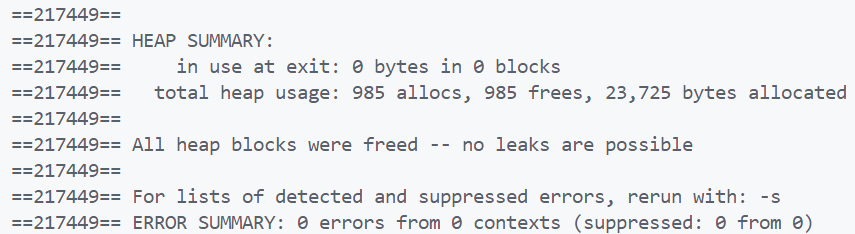
\includegraphics[width=0.8\textwidth]{figures/valgrind_output.png}
    \end{figure}
\end{frame}

\begin{frame}[fragile]{Testing and Analysis}
    \framesubtitle{Word Count Correctness}
    \begin{itemize}
        \item We will use the following script to compare the output of our word count program with the expected output.
    \end{itemize}
    \begin{lstlisting}[language=bash]
word_count() {
    awk '{for(i=1;i<=NF;i++) wc[$i]++} END {for(word in wc) print word, wc[word]}' $@ | sort
}
# Run the wordcount program and calculate execution time
start_time=$(date +%s.%N)
./wordcount tests/1.in > tests-out/1.out
end_time=$(date +%s.%N)
wordcount_time=$(echo "$end_time - $start_time" | bc)

# Use the word_count function to process the file and save the result
word_count tests/1.in > tests/1.out

# Sort the output of the wordcount program
sort tests-out/1.out -o tests-out/1.out

# Compare the results of the wordcount program and the word_count function
if diff -q tests-out/1.out tests/1.out > /dev/null; then
    result=$(tput setaf 2)correct$(tput sgr0)  # Green "correct"
else
    result=$(tput setaf 1)incorrect$(tput sgr0)  # Red "incorrect"
fi

# Print the result
printf "test1 %-10s %.4f s\n" $result $wordcount_time
    \end{lstlisting}
    \note{You can save the script as \textbf{test.sh} and run it with the following command: \textbf{bash test.sh}.}
\end{frame}

\begin{frame}[fragile]{Testing and Analysis}
    \framesubtitle{Efficiency of Multithreaded Map and Reduce}
    \begin{itemize}
        \item First, we will adjust the code in \textbf{wordcount.c} to allow it to adjust the number of map threads and reduce threads based on external parameters.
    \end{itemize}
    \begin{lstlisting}
int main(int argc, char *argv[]) {
    int map_num = 10;
    int reduce_num = 10;
    char **new_argv = malloc(sizeof(char *) * argc);
    int new_argc = 0;

    for (int i = 0; i < argc; i++) {
        if (strcmp(argv[i], "--map") == 0 && i + 1 < argc) {
            map_num = atoi(argv[++i]);
        } else if (strcmp(argv[i], "--reduce") == 0 && i + 1 < argc) {
            reduce_num = atoi(argv[++i]);
        } else {
            new_argv[new_argc++] = argv[i];
        }
    }

    MR_Run(new_argc, new_argv, Map, map_num, Reduce, reduce_num, MR_DefaultHashPartition);
    free(new_argv);
}
    \end{lstlisting}
    \note{This code allows the user to specify the number of map threads and reduce threads using the \textbf{--map} and \textbf{--reduce} parameters.}
\end{frame}

\begin{frame}[fragile]{Testing and Analysis}
    \framesubtitle{Efficiency of Multithreaded Map and Reduce.Cond}
    \begin{itemize}
        \item Then, we adjust the test script, run the script on a longer text (containing 4000 lines, more than 250,000 words), check the correctness and record the time.
    \end{itemize}
    \begin{lstlisting}[language=bash]
for i in {1..4}
do
    map_values=(1 10 100)
    reduce_values=(1 10 100)

    if [ $i -lt 3 ]; then
        # Run the wordcount program and calculate execution time
        start_time=$(date +%s.%N)
        ./wordcount tests/$i.in > tests-out/$i.out
        end_time=$(date +%s.%N)
        wordcount_time=$(echo "$end_time - $start_time" | bc)

        # Use the word_count function to process the file and save the result
        word_count tests/$i.in > tests/$i.out

        # Sort the output of the wordcount program
        sort tests-out/$i.out -o tests-out/$i.out

        # Compare the results of the wordcount program and the word_count function
        if diff -q tests-out/$i.out tests/$i.out > /dev/null; then
            result=$(tput setaf 2)correct$(tput sgr0)  # Green "correct"
        else
            result=$(tput setaf 1)incorrect$(tput sgr0)  # Red "incorrect"
        fi
        # Print the result
        printf "test%-2s %-10s %.4f s\n" $i $result $wordcount_time
    fi
done
        \end{lstlisting}
\end{frame}

\begin{frame}[fragile]{Testing and Analysis}
    \framesubtitle{Efficiency of Multithreaded Map and Reduce.Cond}
    \begin{minipage}{.41\linewidth}
        \begin{lstlisting}[language=bash, firstnumber=1]
for i in {1..4}
do
    map_values=(1 10 100)
    reduce_values=(1 10 100)
    if [ $i -lt 3 ]; then
        # Same as before
    else
        # Get all files
        files=$(find tests/$i.in -type f -name '*.in')

        # Print the header
        printf "%-10s" "test$i"
        for reduce_value in ${reduce_values[@]}
        do
            printf "%-10s" "reduce=$reduce_value"
        done
        printf "\n"
\end{lstlisting}
        \begin{itemize}
            \item Finally, we divide the long text test data into 300 and 100 parts respectively, as test 3 and test 4, and modify the test script to run tests 3 and 4 nine times each
                  \note[item]{for all combinations of \textit{map\_threads=(1 10 100)} and \textit{reduce\_threads=(1 10 100)}.} % chktex 36
        \end{itemize}
    \end{minipage}
    \hspace{13pt}
    \begin{minipage}{.55\linewidth}
        \begin{lstlisting}[language=bash, firstnumber=last]
        # Test each map parameter value once
        for map_value in ${map_values[@]}
        do
            printf "%-10s" "map=$map_value"
            for reduce_value in ${reduce_values[@]}
            do
                # Run the wordcount program and calculate execution time
                start_time=$(date +%s.%N)
                ./wordcount --map $map_value --reduce $reduce_value $files | sort > tests-out/$i-$map_value-$reduce_value.out
                end_time=$(date +%s.%N)
                wordcount_time=$(echo "$end_time - $start_time" | bc)

                # Print the result
                printf "%-10.4f" $wordcount_time
            done
            printf "\n"
        done
    fi
done
\end{lstlisting}
    \end{minipage}
\end{frame}

\begin{frame}[fragile]{Testing and Analysis}
    \framesubtitle{Efficiency of Multithreaded Map and Reduce.Cond}
    \begin{minipage}{.40\linewidth}
        \begin{itemize}
            \item The results of the test script are shown below:
        \end{itemize}
        \begin{figure}
            \centering
            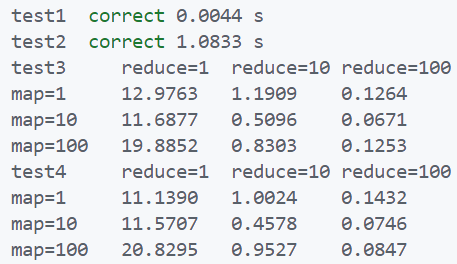
\includegraphics[width=0.9\textwidth]{figures/test_output.png}
        \end{figure}
    \end{minipage}
    \begin{minipage}{.59\linewidth}
        \begin{itemize}
            \item First, it's important to note that when the number of reduce threads is 1, increasing the number of map threads can actually decrease efficiency.
                  \note[item]{This is because the number of reduce threads equals the number of partitions, and a partition can only be accessed by the same map thread at a time.}
            \item Second, increasing the number of reduce threads can always improve performance significantly.
                  \note[item]{Regardless of the number of map threads}
            \item Finally, although the hash function can evenly distribute key-value pairs to each partition, considering the different word frequencies, the load on each node may not be balanced.
                  \note[item]{From an algorithmic perspective, there is still much room for optimization in the program.}
        \end{itemize}
    \end{minipage}
\end{frame}

\end{document}
